\documentclass[11pt,letterpaper]{article}
\usepackage[utf8]{inputenc}
\usepackage[spanish]{babel}
\usepackage{amsmath}
\usepackage{amsfonts}
\usepackage{amssymb}
\usepackage{graphicx}
\usepackage{float}

\usepackage{listings}
\usepackage{color}
\definecolor{miverde}{rgb}{0,0.6,0}
\definecolor{migris}{rgb}{0.9,0.1,0.1}
\definecolor{blue}{rgb}{0,0,0.7}

\lstset{
language=Matlab,
breaklines=true, 
frame=single,
rulesepcolor=\color{migris}, 
commentstyle=\color{miverde},
identifierstyle=\color{blue},
basicstyle=\small\ttfamily}




\title{Precondicionamiento y su utilidad en la generación de mallas con procesos iterativos}
\author{\Large{Universidad Católica San Pablo}
	\\ \large{Maestría en Ciencias de la Computación }
}





\begin{document}

\maketitle


\tableofcontents

\section*{Introducción}

El interes fundamental de este trabajo, se centra en mostrar maneras de como acelerar métodos iterativos para la solución numérica Ax = b, con la matriz A no singular de  $\mathbb{R}^{nxn}$ y  $ b\in\mathbb{R}^n$. la acelaración se consigue con precondicionamiento que será explicado con mas detalles es los siguientes puntos de este trabajo.  Con algún detalle, se consideran precondicionamientos basados en métodos iterativos estacionarios y en factorización LU incompleta

Otro punto a tratar en este trabajo, es la importancia de los metodos iterativos en la generación de mallas, como caso particular se mostrará la generación de malla en 2D. La técnica fundamental para generar este tipo de malla, es la deformación de una malla cartesiana inicial y su posterior alineación con sus fronteras internas.


\section{Precondicionamiento}

\subsection{Historia}

El término \textbf{precondicionamiento} parece haber sido utilizado por primera vez en 1948 por \textbf{Alan Turing}, en el artículo: \textit{El efecto de los errores de redondeo en los métodos de solución directa}. Sin embargo, el primer uso del término en relación con los métodos iterativos se encuentra en un documento de \textbf{D. Evans} sobre la aceleración que aplicaba el ruso \textbf{Chebyschev} en el método de SSOR en 1968.

\textbf{Lamberto Cesari} en 1937 tenía un concepto de precondicionamiento como un medio para poder reducir el \textbf{número condicionante} y así mejorar la convergencia de un proceso iterativo, su idea fue usar un polinomio p(A) de bajo grado aplicada al sistema lineal 
\[
 Ax = b \tag{1} % \label{eq:1}
\]

así  \[ p(A)Ax = p(A)b \] sería un sistema lineal precondicionado, donde A es una matriz de orden $n$ simétrica y definida positiva.

El precondicionar un sistema lineal es una de las principales fuentes para obtener resultados más eficientes computacionalmente. Es así que en los últimos años se ha desarrollado una mayor investigación con respecto a los métodos de solución directa e incluso sobre el subespacio de Krylov.


\subsection{Formulación Matemática}

El término \textbf{precondicionamiento} se refiere a transformar el sistema lineal $(1)$ en otro con propiedades más favorables en cuanto a la solución iterativa y que siga manteniendo la solución \textbf{x}. Un precondicionador es una matriz \textbf{M} que efectúa tal transformación. Para la matriz A del sistema (1), el número condicionante \textbf{cond(A)} se define como:

\vspace{0.1cm}
\[ 
	cond(A) = ||A|| \hspace{0.1cm} ||A^{-1}||
\]

Luego de pre multiplicar al sistema lineal por la matriz \textbf{M} se debería verificar lo siquiente

\[ 
	 MAx = Mb \hspace{0.5cm}, \hspace{0.2cm} cond(MA) < cond(A) 
\]

Esta desigualdad es fundamental para garantizar al favorecimiento de los métodos iterativos, siempre que sea convergente. El mejor precondicionador para el sistema $(1)$ sería $M = A^{-1}$ pues con $cond(A^{-1}A) = cond(I) = 1$ sería el óptimo y así el sistema convergería en tan sólo una interación, pero el problema es calcular el coste computacional de  $A^{-1}$, esto equivaldría a calcular \textbf{$A^{-1}$} por algún método directo. Es por ello que se debe buscar un \textbf{$M \approx A^{-1}$} sin coste elevado.

Para garantizar la convergencia de la matriz A, es suficiente mostrar que su radio espectral $\rho$ es menor a la unidad, matemáticamente  $\rho(A) < 1$. 

Si en la ecuación $(1)$ hacemos $A = M - N$ donde $M$ es una matriz no singular, entonces

\begin{center}
\bgroup\obeylines
$ (M - N)x = b $
$  Mx = Nx + b $
$  x = M^{-1}Nx + M^{-1}b $
$  x = M^{-1}(M - A) + M^{-1}b $
$  x = (I - M^{-1}A)x + M^{-1}b $
\egroup
\end{center}

donde $I$ es la matriz indentidad de orden $n$. En este caso para que el sistema linea converja, se debe cumplir que $\rho(I - M^{-1}A) < 1$. Además mientras el radio espectral sea más cerca a cero entonces la velocidad de convergencia será mayor. 

\vspace{0.2cm}
Los precondicionadores deben cumplir principalmente dos propiedades:
\begin{itemize}
\item Facilidad de implementación (bajo coste computacional).
\item Debe mejorar la convergencia del sistema lineal.
\end{itemize}

Cabe resaltar que los precondicionadores no solamente se obtienen multiplicando por una matriz a la izquierda, sino también por la derecha e incluso por ambos lados.

\subsection{Principales Precondicionadores}

Dentro de los precondicionadores podemos distinguir dos grupos: los explícitos y los implícitos.

\begin{enumerate}
\item \textbf{Precondicionadores Explícitos:} Se busca encontrar una matriz $M$ normalmente a partir de una factorización aproximada, como ejemplo de precondicionadores implícitos tenemos a Jacobi (diagonal), el SSOR, Gradiente Conjugado y las factorizaciones incompletas (Cholesky).

\item \textbf{Precondicionadores Implícitos:} Se construyen calculando directamente $M \approx A^{-1}$, aquí se encuentran los precondicionadores polinomiales e inversa aproximada de $A$.
\end{enumerate}
 

\section{Métodos Iterativos}


La importancia de los métodos iterativos en álgebra lineal se deriva de un simple hecho: los métodos directos requieren de $O(n^{3})$, mientras que los métodos iterativos pueden llegar a requerir solamente $O(n)$. Es así que para matrices con $n > 10^{3}$ se va volviendo intratable el no pensar resolverlo con un algoritmo iterativo. 
Aunque los métodos iterativos requieren menos almacenamiento no tienen la fiabilidad de los métodos directos en cuanto a precisiones de solución se requiere. 

En algunas aplicaciones, los métodos iterativos fallan y es donde el precondicionamiento es necesario, lamentablemente no siempre es suficiente, para lograr la convergencia en un tiempo razonable.
Mientras que los métodos directos están practicamente basados en alguna actualización de la eliminación gaussiana, mientras que los métodos iterativos comprende una gran variedad de técnicas, que van desde métodos verdaderamente iterativos, como el Jacobi clásico, Gauss-Seidel e iteraciones $SOR$ al subespacio de Krylov , que teóricamente convergen en un número finito de pasos.

Por ejemplo, cuando A es definida positiva y simétrica (hermitiana en el caso complejo) el método del Gradiente Conjugado resuelve el sistema $(1)$ muy rápido bajo ciertas condiciones con respecto a sus autovalores.


\subsection{Precondicionadores}

La velocidad de convergencia de los métodos iterativos depende de las propiedades espectrales de la matriz del sistema. Así si M es una matriz invertible que se aproxima de cierta manera a la matriz del sistema, A, los
sistemas
\[Ax = B\]
\[M^{-1}Ax = M^{-1}B\]
tienen las mismas soluciones. No obstante, es posible que las propiedades espectrales de $M^{-1}A$ sean más favorables que las de A. Al sistema
\[M^{-1}Ax = M^{-1}B\]
se le llama sistema precondicionado por la izquierda. Hay otras posibles estrategias para el precondicionado de un sistema como usar un precondicionador por la derecha o combinar iteraciones de distintos métodos iterativos.

Una posible elección de M, que se denomina precondicionador del sistema, es el precondiconador de Jacobi donde M = diag(A).

Otro tipo de precondicionadores, en general, más eficientes son los basados
en descomposiciones LU incompletas de la matriz A.


\section{Generación de Mallas}
En esta sección explicaremos conceptos previos para la generación de mallas, los cuales nos ayudaran a entenderentender la problemática generada, y cómo es que podemos aplicar un m\'etodo de precondicionamiento para agilizar la generaci\'on de mallas.

\subsection{¿Qué es Generación de Mallas?}

%% Breve explicación de en que consiste grid generation y para que se usa %%%%%%%%%%%%%%%%
La idea principal en la generacion de mallas, esta dada en la idea de mallar un espacio dado algunos limites dado un dominio, por ejemplo el ala de un avion. Existen técnicas muy generales, capaces de generar mallas en geometrías complejas, como las de frente de avance o las de Delaunay-Voronoï, que presentan un coste computacional elevado. Por contra, métodos algebraicos generan la malla a una gran velocidad, pero son incapaces de mallar geometrías de cierta complejidad. La geometría del dominio, el coste computacional y la capacidad de control que queramos tener sobre la malla será lo que nos haga decidir por unos u otros métodos.\\

Las mallas se clasifican de acuerdo a su estructura en dos tipos: mallas estructuradas y mallas no estructuradas. La diferencia básica entre una malla estructurada y una malla no estructurada radica en la forma de agrupar los datos que describen la malla. Estas a su vez se subdividen por los métodos empleados en su generación.\\



\begin{itemize}
    \item Métodos de generación de malla estructurada:
     \begin{itemize}
         \item Algebraicos.
         \item Basados en EDPs.
         \item Superposición-deformación de retícula.
         \item Crecimiento estructurado.
    \end{itemize}
    \item Métodos de generación de malla no estructurada:
    \begin{itemize}
         \item Inserción de nodos y posterior conexión: Delaunay.
         \item Generación simultánea de nodos y conectividad: Frente de avance.
         \item Métodos Multibloque.
    \end{itemize}
\end{itemize}

 


%%%%%%%%%%%%%%%%%%%%%%%%%%%%%%%%%%%%%%%%%%%%%%%%%%%%%%%%%%%%%%%%%%%%%%%%%%%%%%%%%%%%%%%%%%

%% Ejemplos -> imágenes sobre generación estructurada y no estructurada, y una breve explicación de ambas
Una malla estructurada consiste generalmente de cuadriláteros, los cuales son formados por un grupo de coordenadas y conexiones que naturalmente son mapeados en elementos de una matriz. Los puntos vecinos dentro de la malla en el espacio físico son los elementos vecinos en la matriz de la malla. De esta manera, un arreglo bidimensional x(i,j) puede usarse para almacenar las coordenadas de los puntos para una malla en 2D.\\

En una malla no estructurada los puntos no pueden ser representados de la misma manera que en las mallas estructuradas, entonces se requiere proveer información adicional para describir la malla. Para representar cualquier punto particular, la conexión con otros puntos puede definirse en la matriz de conectividad.

\begin{figure}[H]
	\begin{minipage}{.49\linewidth}
		\centering
		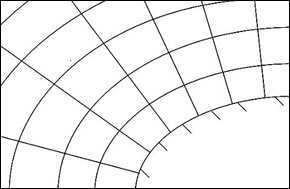
\includegraphics[scale=0.5]{./imgs/mallaEstructurada.jpg}
		\center{a)}
	\end{minipage}
	\begin{minipage}{.49\linewidth}
		\centering
		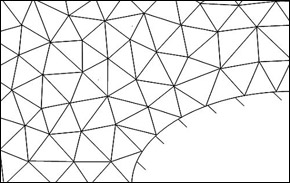
\includegraphics[scale=0.519]{./imgs/mallaNoEstructurada.jpg}
		\center{b)}
	\end{minipage}
	\caption{a) Malla estructurada b) Malla no estructurada.}
\end{figure}

%%%%%%%%%%%%%%%%%%%%%%%%%%%%%%%%%%%%%

%% Mencionar sobre nuestro caso, el estructurado 
El uso de una malla no estructurada es factible en la discretización de geometrías complicadas. Sin embargo, la carencia de una estructura global en una malla no estructurada hace que la aplicación de los algoritmos de solución de barrido de línea sean más difíciles de aplicar que en las mallas estructuradas, impactando directamente en el desarrollo del código computacional haciéndolo más complejo e incrementando el tiempo de cálculo en la solución de problemas en la que se aplique este tipo de discretización.\\

Para nuestro proposito se plantea estudiar mallas estructuradas, la cual a la vez se utilizaran los m\'etodos algebraicos y los m\'etodos basados en PDEs
\\
%%%%%%%%%%%%%%%%%%%%%%%%%%%%%%%%%%%%%%%%%%%%%%%%%

\subsection{Métodos para Generación de Mallas Estructuradas}

%% Tal vez también se pueda mencionar los de mapeo simple, los que haces cambio de variable y ya
Generalmente, para fen\'omenos f\'isicos que tienen lugar en geometr\'ias sencillas, por ejemplo, una cavidad rectangular y la secci\'on transversal de un tubo, se elige un sistema coordenado ortogonal adecuado. Estos sistemas coordenados no necesitan transformación alguna, es decir, el plano físico es igual al plano computacional. Sin embargo, cuando la geometría ya no puede ser representada por los sistemas coordenados ortogonales, es necesario realizar una transformaci\'on que permita mapear la regi\'on f\'isica arbitraria a una regi\'on computacional regular.\\

Para ilustrar los conceptos b\'asicos del mapeo se considera un dominio físico bidimensional en coordenadas cartesianas $x,y$ y un dominio computacional en coordenadas cartesianas $\xi,\eta$. La transformaci\'on entre las coordenadas $x,y$ y $\xi,\eta$ debería ser tal que las fronteras del dominio f\'isico deben coincidir con las coordenadas curvil\'ineas.

\begin{figure}[H]
	\begin{minipage}{.49\linewidth}
		\centering
		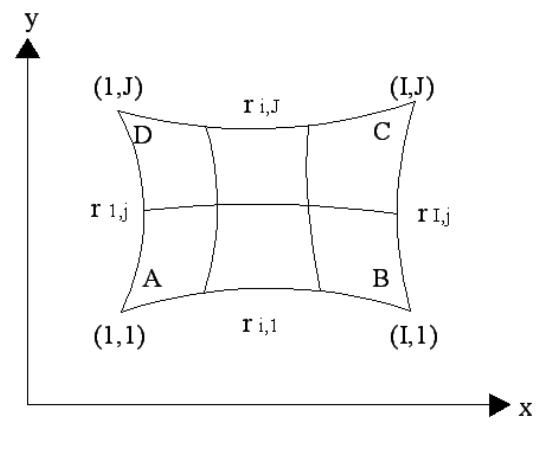
\includegraphics[scale=0.31]{./imgs/planoFisico.jpg}
		\center{a)}
	\end{minipage}
	\begin{minipage}{.49\linewidth}
		\centering
		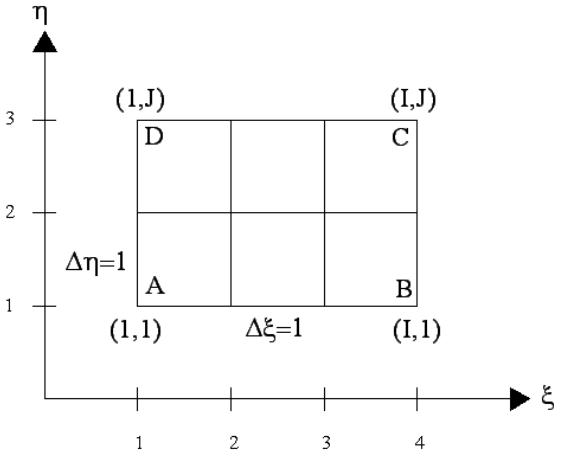
\includegraphics[scale=0.31]{./imgs/planoComputacional.jpg}
		\center{b)}
	\end{minipage}
	\caption{a) Plano F\'isico b) Plano Computacional.}
\end{figure}
%% Breve intro a métodos algebráicos y basados en PDEs %%%%%%%%%%%%%%

Existen muchos métodos para la generación de mallas estructuradas disponibles en la literatura. Fundamentalmente, estos pueden clasificarse en algebraicos y diferenciales. Los algebraicos emplean diferentes tipos de interpolación, así como, expresiones analíticas exactas y son bastante versátiles y rápidos. Los diferenciales, llamados así por que emplean sistemas de ecuaciones diferenciales, son más generales, en contrapartida, requieren un tiempo de calculo mayor y una elaboración matemática más compleja que los métodos algebraicos. 
.

\subsubsection{Métodos Algebraicos Basados en Interpolación}
En estos m\'etodos, se usan ecuaciones algebraicas para relacionar los puntos de malla del dominio f\'isico con el dominio computacional. Una vez definida la geometr\'ia del dominio f\'isico y el dominio computacional construido, la malla en el dominio físico será obtenida por ecuaciones algebraicas. La base de estos m\'etodos es el uso de t\'ecnicas de interpolaci\'on y relaciones algebraicas exactas, lo cual permite la obtenci\'on r\'apida de la malla. Esta es la mayor ventaja de los m\'etodos algebraicos. 	
		\\
		%%%%%%%%%%%%%%%%%%%%%%%%%%%%%%%%%%%%%%%%%%%%%%%%%%%%%%%%%%%%%%%%

		%% Métodos basados en PDEs %%%%%%%%%%%%%%%%%%%%%%%%%%%%%%%%%%%%%
		%% Mencionar tal vez el hiperbólico, pero hacer énfasis en el
		%% elíptico, y mencionar que es el que usamos en nuestro caso
\subsubsection{Métodos Basados en PDEs}
En estos métodos se resuelve un sistema de EDP's para localizar los puntos en el interior del dominio físico, esto es, para generar la malla, pueden clasificarse en sistemas elípticos, parabólicos e hiperbólicos, de acuerdo al tipo de ecuación diferencial que se utiliza para generar la malla.\\

%%%%%%%%%%%%%%%%%%%%%%%%%%%%%%%%%%%%%%%%%%%%%%%%%%%%%%%%%%%%%%%%
\subsubsection{Relación de Transformaci\'on}
A continuacion se muestra la relaci\'on de transformaci\'on entre ambos planos:

\begin{center}
$\xi=\xi(x,y,z),\eta=\eta(x,y,z),\zeta=\zeta(x,y,z)$

$\left[\begin{array}{ccc}
\frac{\partial u}{\partial x} & \frac{\partial u}{\partial y} & \frac{\partial u}{\partial z}\\
\frac{\partial v}{\partial x} & \frac{\partial v}{\partial y} & \frac{\partial v}{\partial z}\\
\frac{\partial w}{\partial x} & \frac{\partial w}{\partial y} & \frac{\partial w}{\partial z}
\end{array}\right]=\left[\begin{array}{ccc}
\frac{\partial u}{\partial\xi} & \frac{\partial u}{\partial\eta} & \frac{\partial u}{\partial\zeta}\\
\frac{\partial v}{\partial\xi} & \frac{\partial v}{\partial\eta} & \frac{\partial v}{\partial\zeta}\\
\frac{\partial w}{\partial\xi} & \frac{\partial w}{\partial\eta} & \frac{\partial w}{\partial\zeta}
\end{array}\right]\left[\begin{array}{ccc}
\frac{\partial\xi}{\partial x} & \frac{\partial\xi}{\partial y} & \frac{\partial\xi}{\partial z}\\
\frac{\partial\eta}{\partial x} & \frac{\partial\eta}{\partial y} & \frac{\partial\eta}{\partial z}\\
\frac{\partial\zeta}{\partial x} & \frac{\partial\zeta}{\partial y} & \frac{\partial\zeta}{\partial z}
\end{array}\right]$

$J=\left[\begin{array}{ccc}
\frac{\partial\xi}{\partial x} & \frac{\partial\xi}{\partial y} & \frac{\partial\xi}{\partial z}\\
\frac{\partial\eta}{\partial x} & \frac{\partial\eta}{\partial y} & \frac{\partial\eta}{\partial z}\\
\frac{\partial\zeta}{\partial x} & \frac{\partial\zeta}{\partial y} & \frac{\partial\zeta}{\partial z}
\end{array}\right]J^{-1}=\left[\begin{array}{ccc}
\frac{\partial x}{\partial\xi} & \frac{\partial x}{\partial\eta} & \frac{\partial x}{\partial\zeta}\\
\frac{\partial y}{\partial\xi} & \frac{\partial y}{\partial\eta} & \frac{\partial y}{\partial\zeta}\\
\frac{\partial z}{\partial\xi} & \frac{\partial z}{\partial\eta} & \frac{\partial z}{\partial\zeta}
\end{array}\right]$

\end{center}	
\subsection{Sobre los Métodos Usados}

	En nuestra implementaci\'on decidimos seguir el procedimiento propuesto en varios libros y papers. Seguimos el 
	siguiente procedimiento: 

	\begin{itemize}
		\item[*] \textbf{ Uso de un generador algebraico }
		\\
		Usamos un generador basado en la Interpolaci\'on Transfinita. La malla generada se usar\'a como condici\'on 
		inicial para nuestro generador basado en PDEs.
		%%%%
		\item[*] \textbf{ Discretizaci\'on de las ecuaciones del generador el\'iptico }
		\\
		El generador basado en PDEs usado es el El\'iptico, cuyas ecuaciones son discretizadas y formadas en un 
		m\'etodo iterativo para calcular un grid por medio de la Iteraci\'on de Picard.
		%%%%
		\item[*] \textbf{ Refinamiento de la malla }
		\\ En este \'ultimo paso usamos el generador El\'iptico discretizado para as\'i poder refinar la malla
		inicial generada por el generador algebraico.
	\end{itemize}

	Acontinuaci\'on pasamos a describir los m\'etodos usados.

\subsubsection{Método Algebraico de Interpolación Transfinita}
En nuestra implementaci\'on usamos el generador algebraico basado en Interpolaci\'on Transfinita. Este puede ser formulado como sigue :
		%
		\begin{gather*}
			x( \xi, \eta ) = ( 1 - \xi ) x_{l} + \xi x_{r} + ( 1 - \eta ) x_{b} + \eta x_{t} - \hdots \\
							 ( 1 - \eta ) ( 1 - \xi ) x_{b}(0) - ( 1 - \xi ) \eta x_{t}(0) - \hdots \\
							 ( 1 - \eta ) \xi x_{b}(1) - \eta \xi x_{t}(1)
			\\
			y( \xi, \eta ) = ( 1 - \xi ) y_{l} + \xi y_{r} + ( 1 - \eta ) y_{b} + \eta y_{t} - \hdots \\
							 ( 1 - \eta ) ( 1 - \xi ) y_{b}(0) - ( 1 - \xi ) \eta y_{t}(0) - \hdots \\
							 ( 1 - \eta ) \xi y_{b}(1) - \eta \xi y_{t}(1)
		\end{gather*}
		Donde, $x_l(\eta)$, $y_l(\eta)$, $x_r(\eta)$, $y_r(\eta)$, $x_b(\xi)$, $y_b(\xi)$, $x_t(\xi)$, $y_t(\xi)$ son las
		fronteras de la geometr\'ia expresadas como funci\'on de $ \xi $ y $ \eta $, las coordenadas en el espacio de 
		c\'omputo.
		\\
		En nuestro caso, cargamos la geometr\'ia de ejemplo mostrada en la siguiente figura :
		\begin{figure}[H]
			\centering
			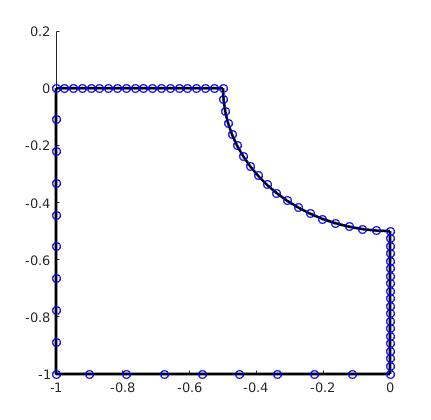
\includegraphics[scale=0.39]{./imgs/img_geometry.jpg}
			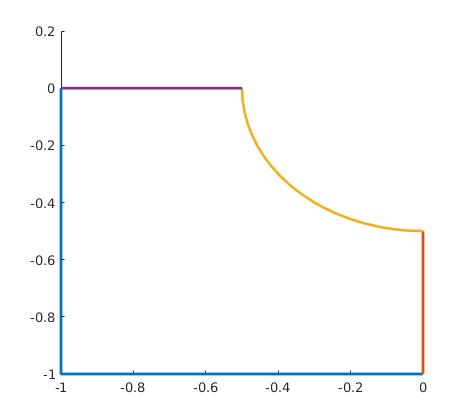
\includegraphics[scale=0.39]{./imgs/img_geometry_boundaries.jpg}
			\caption{Geometr\'ia de prueba}
			\label{fig:img_geometry_boundary}
		\end{figure}
		Esta geometr\'ia est\'a dada en forma de puntos, por lo que no tenemos expresiones anal\'iticas para las fronteras.
		Para esto, expresamos las fronteras como funciones lineales en trozos, haciendo que cada frontera sea definida por un conjunto de subfunciones tipo segmento de recta definidas por los puntos que definen la frontera. Esto se expresa como lo siguinte:
		\begin{gather*}
			x(q) = 
			\begin{cases}
				x_{i}(q) = x(i) + q \lbrace x(i + 1) - x(i) \rbrace
			\end{cases}
			\\
			y(q) = 
			\begin{cases}
				y_{i}(q) = y(i) + q \lbrace y(i + 1) - y(i) \rbrace
			\end{cases}
			\\
			q = {\xi, \eta}
		\end{gather*}
		%
		Al aplicar este m\'etodo a la geometr\'ia dada, obtenemos los siguientes resultados.
		\begin{figure}[H]
			\begin{minipage}{.49\linewidth}
				\centering
				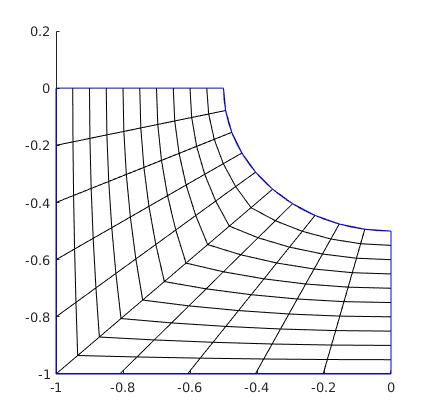
\includegraphics[scale=0.41]{./imgs/img_alg_generator_size_10.jpg}
				\center{a)}
			\end{minipage}
			\begin{minipage}{.49\linewidth}
				\centering
				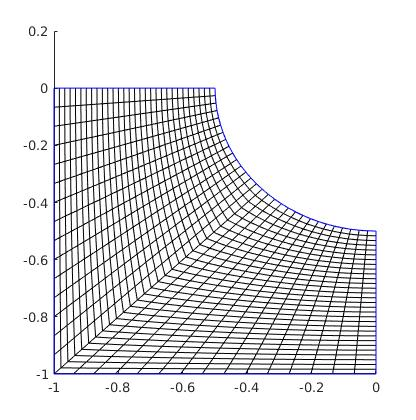
\includegraphics[scale=0.41]{./imgs/img_alg_generator_size_30.jpg}
				\center{b)}
			\end{minipage}
			\caption{Grid generado para la geometr\'ia de prueba usando el m\'etodo algebraico, size de a)10 y b)30}
			\label{fig:img_grid_algebraic}
		\end{figure}
\subsubsection{Método Basado en PDEs Elípticas}
Para poder refinar la malla generada por el generador algebraico usamos un generador basado en PDEs. El generador es del tipo el\'iptico, el cu\'al define la nueva grilla como la soluci\'on a la siguiente PDE :
		\begin{gather*}
		%
			\xi_{xx} + \xi_{yy} = 0 \\
			\eta_{xx} + \eta_{yy} = 0 \\
		%
		\end{gather*}
		\'Estas PDEs las transformamos del espacio $x,y$ al espacio $\xi, \eta$, lo cu\'al nos deja un problema de frontera ( con fronteras $x(\xi,\eta)$, $y(\xi,\eta)$ ) definido por las siguientes ecuaciones :
		\begin{gather*}
		%
			( x_{\eta \eta}^{2} + y_{\eta \eta}^{2} )x_{\xi \xi} 
				- 2 ( x_{\xi} x_{\eta} + y_{\xi} y_{\eta} ) x_{\xi \eta}
				+ ( x_{\xi \xi}^{2} + y_{\xi \xi}^{2} )x_{\eta \eta} 
			\\
			( x_{\eta \eta}^{2} + y_{\eta \eta}^{2} )y_{\xi \xi} 
				- 2 ( x_{\xi} x_{\eta} + y_{\xi} y_{\eta} ) y_{\xi \eta}
				+ ( x_{\xi \xi}^{2} + y_{\xi \xi}^{2} )y_{\eta \eta} 
		%
		\end{gather*}
		%
		Al discretizarlas obtenemos las siguientes ecuaciones :
		\begin{gather*}
			\alpha_{ij} ( x_{i+1,j} - 2 x_{i,j} + x_{i-1,j} ) + \gamma_{ij} ( x_{i, j + 1} - 2 x_{i, j} + x_{i,j-1} ) - \hdots \\
				 0.5 \beta_{ij} ( x_{i+1,j+1} - x_{i+1,j-1} - x_{i-1,j+1} + x_{i-1,j-1} ) = 0
			\\
			\alpha_{ij} ( y_{i+1,j} - 2 y_{i,j} + y_{i-1,j} ) + \gamma_{ij} ( y_{i, j + 1} - 2 y_{i, j} + y_{i,j-1} ) - \hdots \\
				 0.5 \beta_{ij} ( y_{i+1,j+1} - y_{i+1,j-1} - y_{i-1,j+1} + y_{i-1,j-1} ) = 0
		\end{gather*}
		\\
		Donde:
		\begin{gather*}
		%
			 \xi = \frac{i}{N_{\xi}},\eta = \frac{j}{N_{\eta}}
			 \\
			 \alpha_{ij} = 0.25 ( ( x_{i,j+1} - x_{i,j-1} )^{2} + (y_{i,j+1} - y_{i,j-1})^{2} )
			 \\
			 \beta_{ij} = 0.25 ( ( x_{i,j+1} - x_{i,j-1} ) ( x_{i+1,j} - x_{i-1,j} ) + ( y_{i,j+1} - y_{i,j-1} ) ( y_{i+1,j} - y_{i-1,j} ) )
			 \\
			 \gamma_{ij} = 0.25 ( ( x_{i+1,j} - x_{i-1,j} )^{2} + (y_{i+1,j} - y_{i-1,j})^{2} )
		%
		\end{gather*}
		%
		Para resolver estas ecuaciones y transformarlas a un sistema lineal hacemos uso de la iteraci\'on de Picard, haciendo que los coeficientes $\alpha, \beta, \gamma$
		sean dependientes de la malla actual, mientras que los otros t\'erminos sean dependientes de la malla siguiente, teniendo lo siguiente ( caso $x$ ) :
		\begin{gather*}
			\alpha_{ij}^{k} ( x_{i+1,j}^{k+1} - 2 x_{i,j}^{k+1} + x_{i-1,j}^{k+1} ) + \gamma_{ij}^{k} ( x_{i, j + 1}^{k+1} - 2 x_{i, j}^{k+1} + x_{i,j-1}^{k+1} ) - \hdots \\
				 0.5 \beta_{ij}^{k} ( x_{i+1,j+1}^{k+1} - x_{i+1,j-1}^{k+1} - x_{i-1,j+1}^{k+1} + x_{i-1,j-1}^{k+1} ) = 0
		\end{gather*}
		Con lo cu\'al podemos formar el sistema $Az = b$, donde $A$ es la forma matricial de las ecuaciones anteriores luego de aplicar el stencil mostrado en la figura siguiente, $z$ es la representaci\'on en vector columna de la grilla en la siguiente iteraci\'on-refinamiento y $b$ se obtiene de aplicar las condiciones de frontera.
		\begin{figure}[H]
			\centering
			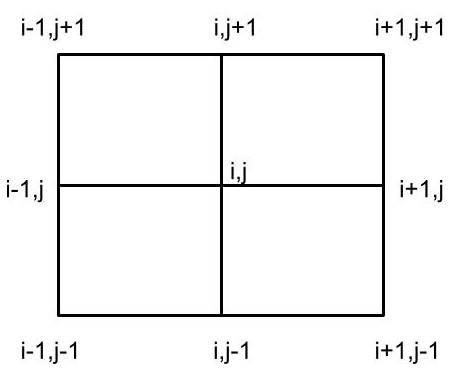
\includegraphics[scale=0.5]{./imgs/img_stencil.jpg}
			\caption{Stencil a aplicar a las ecuaciones discretizadas del generador el\'iptico}
			\label{fig:img_stencil}
		\end{figure}
		Implementamos el generador el\'iptico en MATLAB, lo cu\'al nos dio los siguientes resultados al usar la malla del generador algebraico de la geometr\'ia de ejemplo como condici\'on inicial.
		
\begin{figure}[H]
	\begin{minipage}{.49\linewidth}
		\centering
		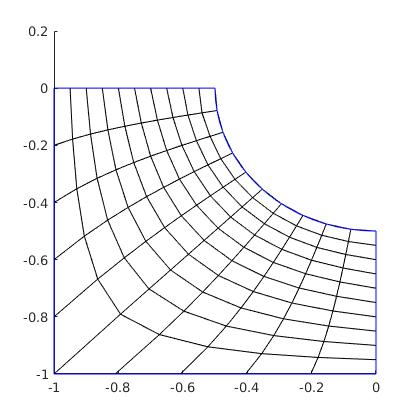
\includegraphics[scale=0.41]{./imgs/img_elliptic_generator_size_10.jpg}
		\center{a)}
	\end{minipage}
	\begin{minipage}{.49\linewidth}
		\centering
		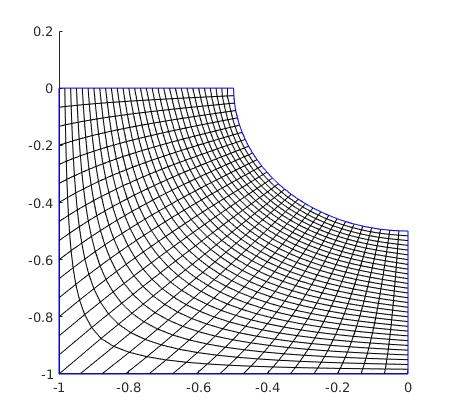
\includegraphics[scale=0.41]{./imgs/img_elliptic_generator_size_30.jpg}
		\center{b)}
	\end{minipage}
	\caption{Grid generado para la geometr\'ia de prueba usando el generador el\'iptico, size de a)10 y b)30}
			\label{fig:img_grid_algebraic}
\end{figure}
	
\section{Resultados}
En el desarrollo del presente trabajo verificamos la importancia de usar precondicionamiento al momento de resolver un sistema de ecuación lineal para la generación de una malla, para este propósito se uso el método de gauss seidel por bloque como matriz de precondicionamiento, y como se podrá observar en la siguiente figura ambas mallas son generadas correctamente con ambos métodos, con la diferencia que el método de gauss seidel por bloque converge con mucho menos iteraciones que el método de gauss seidel tradicional.

\begin{figure}[H]
	\begin{minipage}{.49\linewidth}
		\centering
		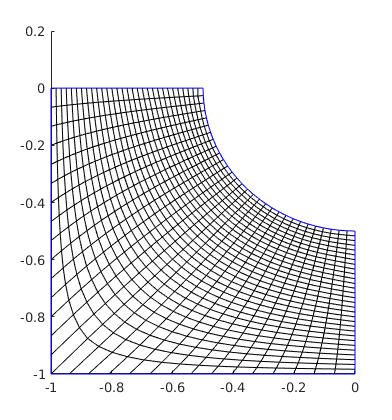
\includegraphics[scale=0.44]{./imgs/GSBloque.jpg}
		\center{a)}
	\end{minipage}
	\begin{minipage}{.49\linewidth}
		\centering
		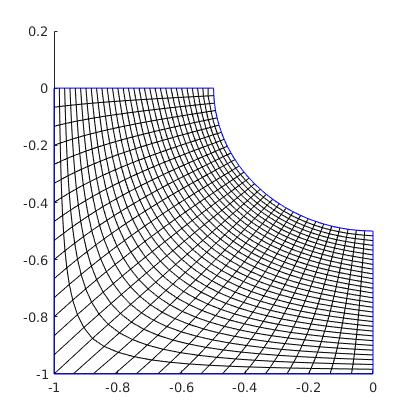
\includegraphics[scale=0.44]{./imgs/GS.jpg}
		\center{b)}
	\end{minipage}
	\caption{a)Gauss seidel por bloque. Converge con 13 iteraciones b)Gauss seidel. Converge con 715 iteraciones}
\end{figure}


\clearpage
\begin{thebibliography}{10}
\bibitem{Benzi} 
MICHELE BENZI:
\textit{Preconditioning Techniques for Large Linear
Systems: A Survey - }
Mathematics and Computer Science Department, Emory University, Atlanta, Georgias, 2002.
 
\bibitem{Saad} 
YOUSEF SAAD:
\textit{Iterative Methods for Sparse Linear Systems - } 
second Edition, 2000.
 
\bibitem{Thompson} 
JOE F. THOMPSON, BHARAT K. SONI, NIGEL P. WEATHERILL:
\textit{Handbook of Grid Generation - }
1999.

\bibitem{Lloyd} 
LLOYD N. TREFETHEN, DAVID BAU:
\textit{Numerical Linear Algebra - }
1997.

\end{thebibliography}

\clearpage
\section{Anexos}
\subsection{Código - Gauss Seidel}
\lstinputlisting[language=Matlab]{gs.m}
\subsection{Código - Gauss Seidel por Bloque}
\lstinputlisting[language=Matlab]{Bgs.m}

\end{document}
